\chapter{Gestión y control de concurrencia}

En el anterior tema vimos como trabajaban las transacciones dentro de un SGBD, pero siempre suponíamos que cada transacción accedía a datos únicamente usados por ella misma. Evidentemente, esto en la vida real casi nunca pasa ya que los usuarios suelen usar muchos datos compartidos. Por este motivo es necesario definir un control sobre el orden en el que se realizan transacciones que afectan a los mismos datos.

Además la gestión de la concurrencia es necesaria por eficiencia, ya que si no existiera y hubiera 100 usuarios conectados, 99 usuarios deberían quedarse esperando a que termine la transacción del otro usuario. Además hay que garantizar la consistencia de la BD, es decir, las ejecuciones concurrentes no deben dejar la BD en un estado inconsistente.

\section{Problemas del acceso concurrente}

\subsection{Anulación de transacción}

\begin{figure}[H]
  \center
  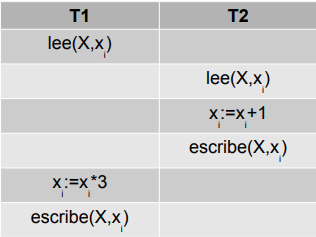
\includegraphics[scale=0.5]{img/22.png}
\end{figure}

Cuando una transacción quiere acceder a un dato que está siendo modificado por otra o cuando es eliminado por otra.

Lo más seguro en estos casos es que el mecanismo de control de concurre anule una de estas transacciones, es decir, le impida al usuario realizar su consulta. Hay muchos algoritmos para decidir cual se anularía, los veremos más adelante.

Fijaros que en esta tabla no hay varias entradas en la misma fila, a diferencia de lo que pasaba en el tema anterior, donde teníamos que \textit{suponer} qué entradas de la misma fila se ejecutaban (de izquierda a derecha, por ejemplo). Eso realmente nunca ocurre ya que la ejecución de las transacciones es no determinista. Si ejecutamos dos transacciones varias veces, es poco probable que nos salga el mismo orden en la tabla.

Si juntamos las dos columnas de la tabla en una sola, nos quedaría una columna totalmente rellena que recibe el nombre de \textbf{ejecución} o \textbf{plan de ejecución}.

\subsection{Estado inconsistente de la BD}

\begin{figure}[H]
  \center
  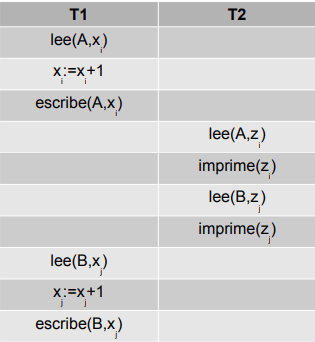
\includegraphics[scale=0.5]{img/23.png}
\end{figure}

La BD puede quedarse en un estado inconsistente si hay transacciones concurrentes que violan tamporalmente las restricciones de la BD. Estas restricciones suelen ser semánticas. Por ejemplo, supongamos en la tabla de arriba que B es clave externa de A, luego no deben tener valores distintos en ningún momento. En la tabla se ve que en la T2, la sentencia \textit{lee(B,$z_j$)}, no estaría referenciando a ningún valor de la tabla o estaría referenciando a un valor incorrecto, ya que $A$, la clave a la que hace referencia, ha cambiado pero $B$ no ha sido actualizado (se actualiza en las tres últimas sentencias).

\begin{figure}[H]
  \center
  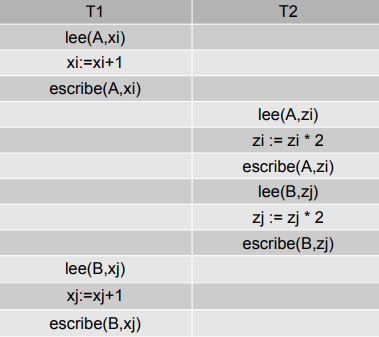
\includegraphics[scale=0.5]{img/24.png}
\end{figure}

En este caso, pasa prácticamente lo mismo que el anterior pero está un poco más escondido.

Para seguir estudiando la concurrencia, necesitamos definir lo que es una \textbf{operación en conflicto}. Primero tenemos que definir lo que es una \textbf{operación}, que no es más que un conjunto de sentencias que hacen uso del mismo átomo y de las mismas variables. Por ejemplo, en la tabla anterior tenemos 4 operaciones distintas: las 3 primeras sentencias, las 3 siguientes, las 3 siguientes otra vez y las 3 últimas. Una operación nunca puede aparecer en dos transacciones distintas. Se dirá que las operaciones están en conflicto si:
\begin{itemize}
\item pertenecen a distintas transacciones
\item acceden al mismo dato, y
\item alguna de ellas ejecuta la orden \textit{escribe()}.
\end{itemize}
Dos operaciones que no modifican el átomo y pertenecen a dos transacciones distintas, pueden ejecutarse simultáneamente. Es decir, las operaciones de \textit{solo lectura} pueden intercalarse.

\section{Ejecuciones concurrentes sin conflicto}

Un SGBD ejecuta transacciones concurrentes asegurando que se va a llegar a ningún conflicto en ninguno de los casos. Sobre una misma transacción, hay muchos planes de ejecución posibles. Debido al gran número de planes, no es posible estudiarlos todos.

Denotamos por \textbf{átomo} a un fragmento de información de la BD  cuyo acceso concurrente debe controlarse. Por ejemplo, en la tabla anterior, un átomo serían los campos A y B, ya que si no controlamos su acceso concurrente existirán escenarios donde se pierda la consistencia de la BD. Un átomo puede ser una tabla, un atributo, una tupla, etc. A menor tamaño del átomo, más difícil de controlar es (hacen falta más recursos). A mayor tamaño, más transacciones tienen que esperar su turno con el átomo.

Recordemos que en las dos transacciones anteriores habíamos detectado 4 operaciones distintas (porque tienen un escribe en la parte de abajo).

\begin{figure}[H]
\centering
\begin{subfigure}{.5\textwidth}
  \centering
  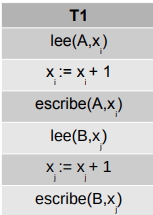
\includegraphics[width=.4\linewidth]{img/25.png}
\end{subfigure}%
\begin{subfigure}{.5\textwidth}
  \centering
  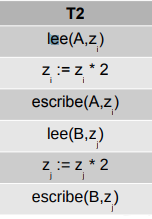
\includegraphics[width=.4\linewidth]{img/26.png}
\end{subfigure}
\end{figure}

Con esas dos transacciones en mente, supongamos que se produce el siguiente plan de ejecución:

\begin{figure}[H]
  \center
  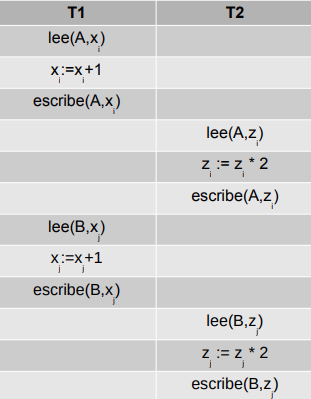
\includegraphics[scale=0.5]{img/27.png}
\end{figure}

¿Sería correcto? Empezando desde el principio, vemos que $A$ y $B$ reciben las mismas actualizaciones, luego la restricción semántica se seguiría manteniendo. También podríamos haber ejecutado T1 entero primero y luego T2 entero.

\begin{figure}[H]
  \center
  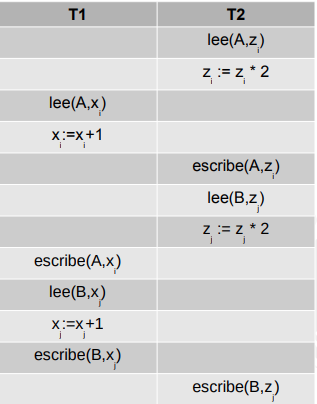
\includegraphics[scale=0.5]{img/28.png}
\end{figure}

¿Es este también correcto? No, ya que al final del plan de ejecución el valor de $A$ sería $A+1$ y el de $B$ sería $2\cdot B$, luego no se mantendría la restricción semántica. Simplemente al ver que las dos primeras operaciones tienen una parte común, debería ponernos en alerta de que seguramente habrá algún error en la consistencia.

Esa ejecución se denominaría \textit{no serializable}. Si el resultado de la ejecución de un conjunto de transacciones concurrentes coincide con la ejecución secuencial de las transacciones, se dice que esa ejecución es \textbf{serializable}.

\section{Operaciones}

\subsection{Operaciones compatibles}

Sean $O_i$ y $O_j$, diremos que son \textbf{operaciones compatibles} si toda ejecución simultánea de ambas da el mismo resultado que la ejecución secuencial de ambas en cualquier orden.

\begin{figure}[H]
\centering
\begin{subfigure}{.5\textwidth}
  \centering
  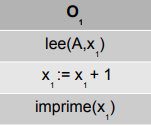
\includegraphics[width=.4\linewidth]{img/29.png}
\end{subfigure}%
\begin{subfigure}{.5\textwidth}
  \centering
  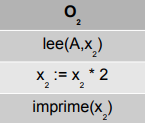
\includegraphics[width=.4\linewidth]{img/30.png}
\end{subfigure}
\caption{¿Son compatibles o incompatibles?}
\end{figure}

Son compatibles ya que la operación \textit{imprime} no altera el valor de $A$, luego son operaciones de sólo lectura.

\begin{figure}[H]
\centering
\begin{subfigure}{.5\textwidth}
  \centering
  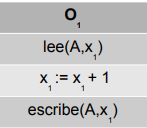
\includegraphics[width=.4\linewidth]{img/31.png}
\end{subfigure}%
\begin{subfigure}{.5\textwidth}
  \centering
  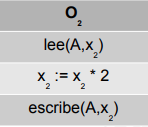
\includegraphics[width=.4\linewidth]{img/32.png}
\end{subfigure}
\caption{¿Son compatibles o incompatibles?}
\end{figure}

Sin embargo, estas operaciones son incompatibles, ya que el siguiente plan de ejcución:

\begin{figure}[H]
  \center
  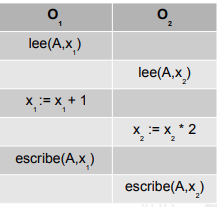
\includegraphics[scale=0.6]{img/33.png}
\end{figure}

el estado sería incorrecto. También pasa si ejecutas primero $O_1$ y luego $O_2$ o viceversa, es decir, no son permutables.

\subsection{Operaciones permutables}

Dos operaciones $O_i$ y $O_j$ son permutables si la ejecución de $O_j$ tras $O_i$ da el mismo resultado que la ejecución de $O_i$ tras $O_j$.

\begin{figure}[H]
\centering
\begin{subfigure}{.5\textwidth}
  \centering
  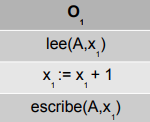
\includegraphics[width=.4\linewidth]{img/34.png}
\end{subfigure}%
\begin{subfigure}{.5\textwidth}
  \centering
  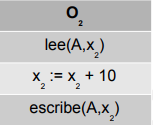
\includegraphics[width=.4\linewidth]{img/35.png}
\end{subfigure}
\caption{¿Son permutables?}
\end{figure}

Sí, porque el valor de $A$ es el mismo independientemente de cuál ejecutes primero. Pero, ¿son compatibles? No. Considera el plan de ejecución siguiente:

\begin{figure}[H]
  \center
  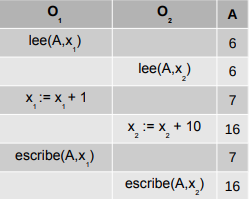
\includegraphics[scale=0.6]{img/36.png}
\end{figure}

\subsection{Ejecuciones serializables}

Queremos coger un plan que ya tengamos hecho y ver si lo podemos expresar mediante operaciones serializables. Esto se lleva a cabo mediante transformaciones sobre la ejecución:
\begin{itemize}
\item Separación de operaciones compatibles: dadas dos operaciones compatibles entrelazadas en transacciones distintas, se cambian por una secuencia de operaciones que den el mismo resultado.
\item Re-ordenación de operaciones permutables: se cambia el orden de ejecución de operaciones permutables. 
\end{itemize}

\textbf{Teorema.} Una condición suficiente para una ejecución serializable es que pueda ser transformada por separación y permutación en una sucesión de transacciones.

\section{Grafo de precedencia}

Para mantener la concurrencia, usamos un \textbf{grafo de precedencia}. Lo podemos ir contruyendo mientras las transacciones van llegando. Nos permite saber qué y quién está haciendo con los átomos.

\begin{itemize}
\item Nodos: transacciones
\item Arcos: restricciones en la ejecución.
\item $T_i$ precede a $T_j$ si, y sólo si, existen dos operaciones no permutables sobre el mismo átomo en las dos transacciones y la operación de $T_i$ es anterior a la de $T_j$.
\item Habrá un arco entre dos transacciones si una precede a otra, y se marca el arco con el nombre del átomo implicado.
\end{itemize}

\begin{figure}[H]
\centering
\begin{subfigure}{.5\textwidth}
  \centering
  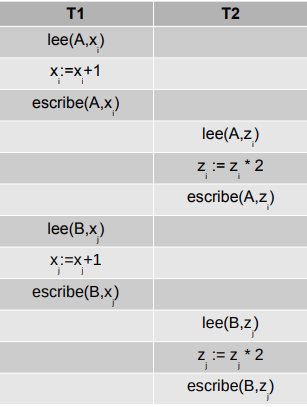
\includegraphics[width=.7\linewidth]{img/37.png}
\end{subfigure}%
\begin{subfigure}{.6\textwidth}
  \centering
  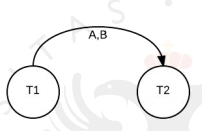
\includegraphics[width=.4\linewidth]{img/38.png}
\end{subfigure}
\end{figure}

\begin{figure}[H]
\centering
\begin{subfigure}{.5\textwidth}
  \centering
  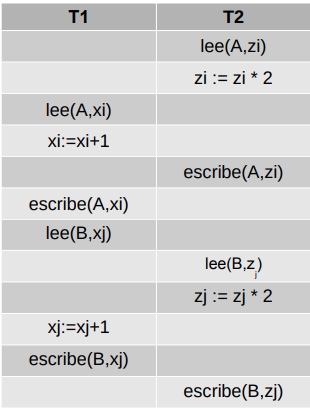
\includegraphics[width=.7\linewidth]{img/39.png}
\end{subfigure}%
\begin{subfigure}{.6\textwidth}
  \centering
  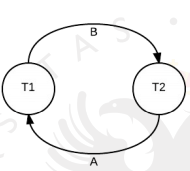
\includegraphics[width=.4\linewidth]{img/40.png}
\end{subfigure}
\end{figure}

\textbf{Teorema.} Condición suficiente para que una ejecución sea serializable es que el grafo de dependencias no presente \underline{\textbf{ciclos dirigidos}}.

\section{Algoritmos de control de concurrencia}

El hecho de que una ejecución sea serializable, permite la creación de ciertos algoritmos que fuerzan ejecuciones serializables en una serie de transacciones. Son técnicas para garantizar el aislamiento de las transacciones y
\begin{itemize}
\item Permitir la ejecución y deshacer las que produzcan conflicto: \textit{técnicas de ordenación por marcas de tiempo}.
\item Evitar ciclos mediante esperas: \textit{técnicas de bloqueo}.
\end{itemize}

\subsection{Técnicas de ordenación por marcas de tiempo}

Cada transacción recibe una marca de tiempo única cuando comienza. A cada átomo $x$, se asocia una referencia a la última transacción que opera sobre él $R(x)$ (la marca que recibe al \textit{start} la transacción)

Recordemos que cada transacción recibe una marca de tiempo inicial cuando hace \textit{start}.

\subsubsection{Ordenación total}

Sean dos transacciones $T_i$ y $T_j$ con $i$ y $j$ marcas de tiempo tales que $i<j$, el algoritmo garantiza que $T_i$ accede antes que $T_j$. Si una operación falla (\textit{ABORT}), se deshace la transacción y se re-lanza más tarde, asignándole a la retrasada una referencia mayor que la de todas las actuales.

\textbf{Problema:} las lecturas concurrentes también se ordenan, sin ser necesario por no ser conflictivas.

\begin{figure}[H]
  \center
  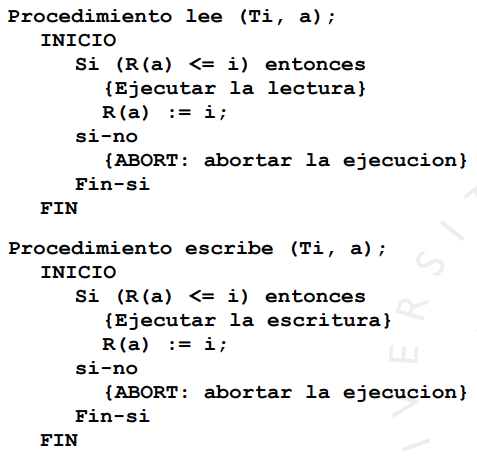
\includegraphics[scale=0.45]{img/41.png}
\end{figure}

Vemos que el algoritmo es muy sencillo, simplemente comprueba que el índice $i$ (marca de tiempo) sea superior (es decir, que pase después) que la referencia a la última transacción que ha operado sobre el átomo $a$, es decir, $R(a)$.

Básicamente lo que hacemos es que si $T_1$ da problemas y hay que abortarla, pues la renombramos a $T_{n+1}$, donde $n$ es el número de transacciones totales, es decir, la mandamos al final para que no de ningún problema.

\subsubsection{Ordenación parcial}

Sólo se ordenan las parejas de operaciones lee/escribe, escribe/lee y escribe/escribe (por eso es parcial). Cada átomo $x$ tiene dos referencias: una para determinar la última transferencia que lo leyó $RR(x)$ y otra para la que lo actualizó $WR(x)$. 

Si una operación falla (\textit{ABORT}), se deshace la transacción y se re-lanza más tarde, asignándole a la retrasada una referencia mayor que la de todas las actuales.

\begin{figure}[H]
  \center
  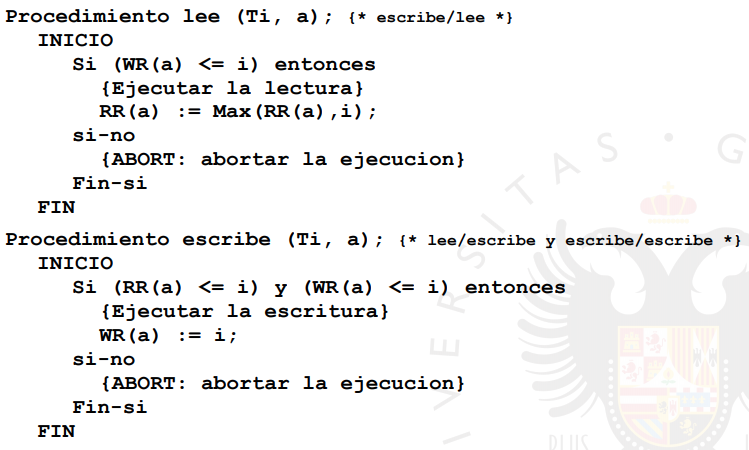
\includegraphics[scale=0.45]{img/42.png}
\end{figure}

\subsubsection{Ordenación parcial multi-versión}

Persigue que las lecturas no aborten una transacción, pero implica que haya distintas versiones de cada átomo. Sólo habrá que buscar la última versión escrita con referencia menor que la de la transacción en curso.

\begin{figure}[H]
\centering
\begin{subfigure}{.5\textwidth}
  \centering
  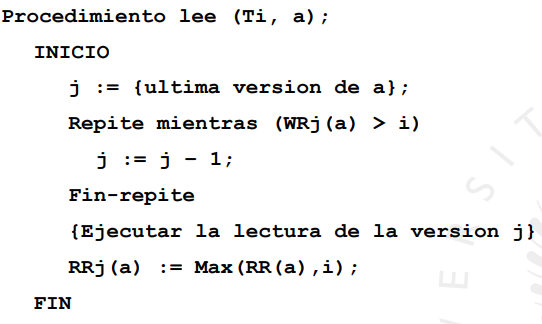
\includegraphics[width=\linewidth]{img/43.png}
\end{subfigure}%
\begin{subfigure}{.5\textwidth}
  \centering
  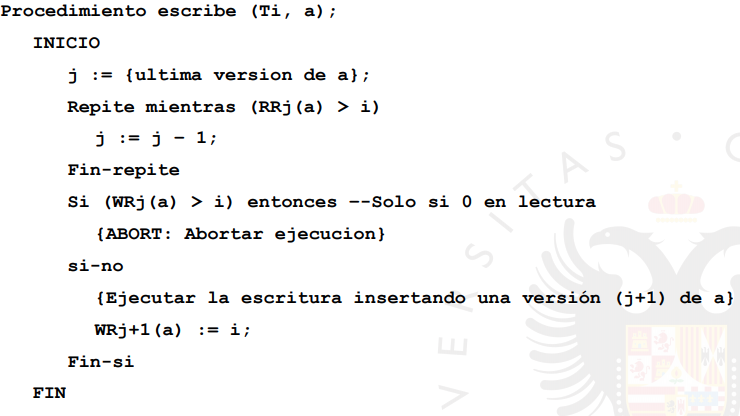
\includegraphics[width=\linewidth]{img/44.png}
\end{subfigure}
\end{figure}

\subsubsection{Control de concurrencia mediante validación}

Las transacciones se dividen en tres fases:
\begin{itemize}
\item Lectura: donde se leen átomos, realizan cálculos y actualizan variables.
\item Validación: se comprueba la validez de los datos.
\item Escritura: se vuelcan los átomos al buffer.
\end{itemize}
Además, para cada transacción, se guardan las marcas de tiempo para inicio, validación y fin.

\subsection{Técnicas de bloqueo}
